\chapter{Introduction}

\section{Motivation}
Logic circuits underpin practically every aspect of modern life in the form of computer chips. It is therefore important that people have the opportunity to learn about and understand logic circuits.

I believe that one of the best ways to learn about logic circuits is to build them, and that the most accessible way of doing that is by using a simulated workbench --- avoiding the cost and knowledge of realising physical circuits. The workbench should be easy to use, but not simplify the simulation to the point where it gives a false impression of how logic gates work. The workbench is not designed to be used by professionals in designing chips, but for casual users looking to learn about logic circuitry.

Projects which attempt to solve the same problem can already be found on the Internet. Two of the best examples I could find were Logic.ly\footnote{http://logic.ly} and CircuitLab\footnote{http://www.circuitlab.com}.

Logic.ly was easy to use but had two major problems. First and foremost, the simulation implemented in Logic.ly over simplified: it does not assign any propagation delay to its components, making it difficult to see what happens in oscillating circuits. Secondly, it is implemented using Adobe Flash. Flash requires a web browser plug-in not included on many devices (notably iOS devices), which reduces Logic.ly's accessibility.

CircuitLab is more aimed at power users and has a much steeper learning curve than most casual users are likely to endure.

\section{Overview of GatePlay}
The main interface of GatePlay can be seen in figure~\ref{fig:interface}. The labelled regions are:

\begin{itemize}
	\item[1] The \textbf{top bar}, which has buttons to download the workbench as an image and to start simulating the circuit. When simulating, the top bar has additional controls such as starting, restarting, and pausing the simulation.
	\item[2] The \textbf{left bar}, which has sliding panels containing the  components available to build circuits with. The user simply drags a gate from the left bar onto the workbench to add it to the circuit.
	\item[3] The \textbf{workbench}, which is where almost all interaction with GatePlay happens. When editing you can move, delete, and draw wires between components. When simulating the values of wires are shown visually on the workbench.
\end{itemize}

GatePlay has a library of standard components which can be used to build circuits. All of the components are implemented as black boxes, even though most of them can be re-implemented using a combination of the simpler components.

\begin{itemize}
	\item \textbf{Input} components such as constant $ON$, $Toggle$ (clicking on a $Toggle$ during simulation will change its value), and $Blinker$ (which flip their value at a constant interval)
	\item \textbf{Gates} implement standard boolean logic functions such as $NOT$, $AND$, and $XOR$
	\item \textbf{Function} components such half adders and full adders
	\item \textbf{Memory} components such as SR latches and D flip-flop  
\end{itemize}

A typical workflow for creating circuits would be:

\begin{enumerate}
	\item Drag the desired components from the left-bar on to the workbench
	\item Wire the components up by left-clicking on output ports, and then left-clicking on an input port. Fixed points can be created along the way by left-clicking on an empty part of the workbench
	\item Entering simulation mode by clicking on the "Start Simulating" button on the top-bar
	\item The simulation can now be paused, resumed, or advanced manually by using the controls in the top-bar
	\item The user may decide to return to editing mode to add, move, or delete components, or re-wire parts of the circuit.
\end{enumerate}

Figure~\ref{fig:dflopflop} shows a D flip-flop being simulated on the workbench. Green wires are $High$ (logical $True$) and red wires are $Low$ (logical $False$). The round components on the left are $Toggle$s; clicking them will change their value and cause the resulting changes to propagate through the circuit.

\begin{figure}[p]
    \centering
    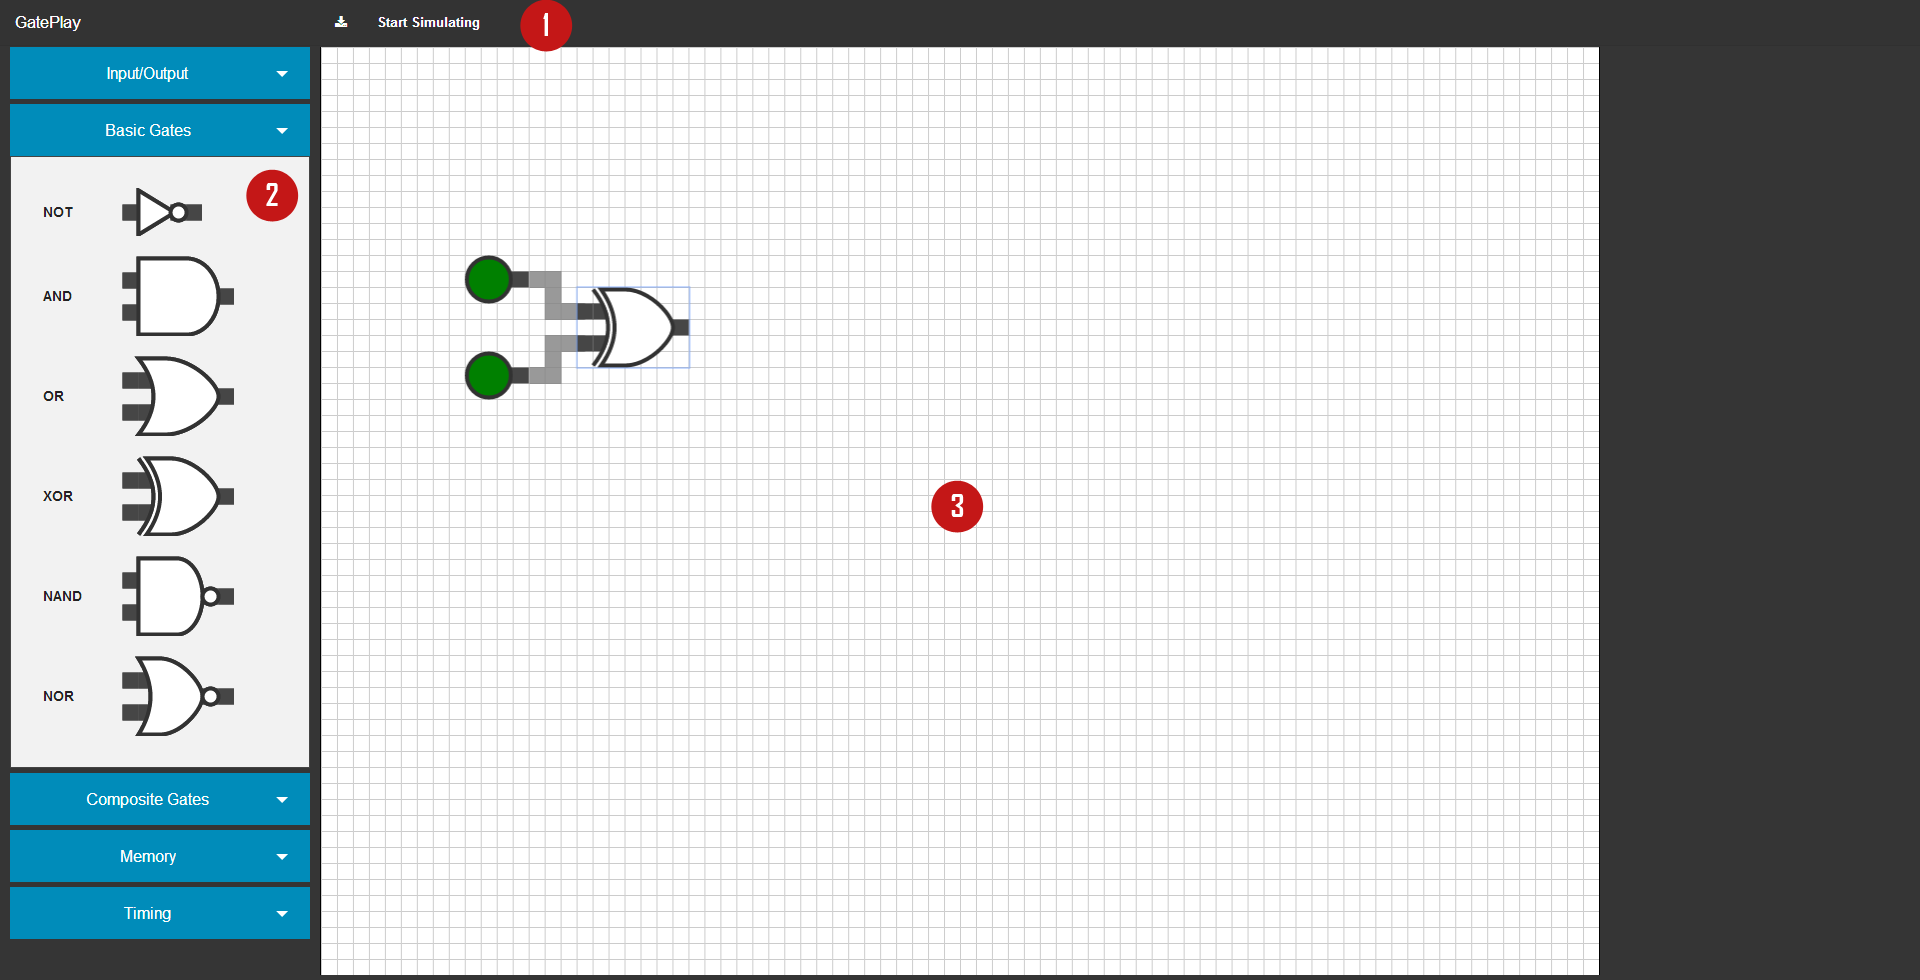
\includegraphics[width=\textheight,angle=90]{labelled.png}
    \caption{Drawing a circuit}
    \label{fig:interface}
\end{figure}

\begin{figure}[p]
    \centering
    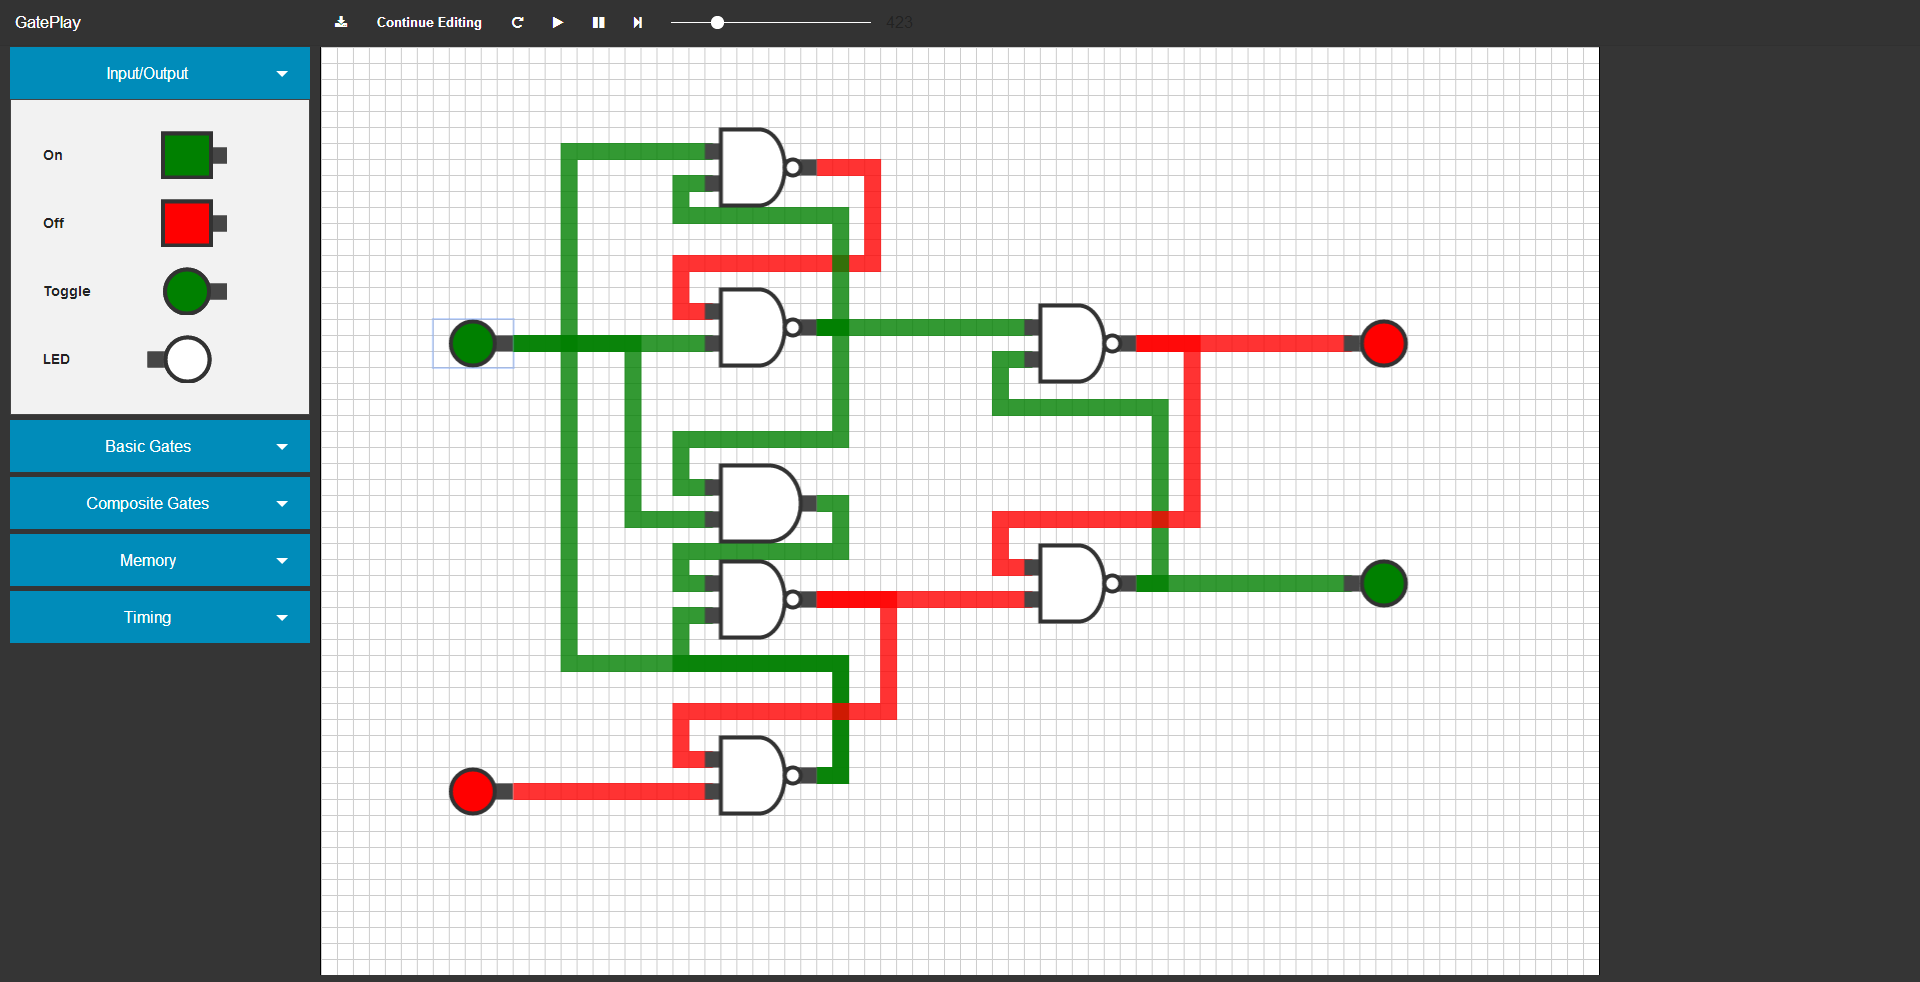
\includegraphics[width=\textheight,angle=90]{dflipflop.png}
    \caption{Simulating a D flip-flop}
    \label{fig:dflopflop}
\end{figure}